\documentclass[12pt]{article}
\usepackage[a4paper,margin=.5in]{geometry}
\usepackage{graphicx}
\usepackage{booktabs}
\usepackage{listings}
\usepackage{color}

\definecolor{dkgreen}{rgb}{0,0.6,0}
\definecolor{gray}{rgb}{0.5,0.5,0.5}
\definecolor{mauve}{rgb}{0.58,0,0.82}

\lstset{frame=tb,
  language=Python,
  aboveskip=3mm,
  belowskip=3mm,
  showstringspaces=false,
  columns=flexible,
  basicstyle={\small\ttfamily},
  numbers=none,
  numberstyle=\tiny\color{gray},
  keywordstyle=\color{blue},
  commentstyle=\color{dkgreen},
  stringstyle=\color{mauve},
  breaklines=true,
  breakatwhitespace=true,
  tabsize=3
}
%\usepackage{subfig}
\usepackage{subcaption}
\usepackage{hyperref}
\hypersetup{
    colorlinks=true,
    linkcolor=blue,
    filecolor=magenta,      
    urlcolor=cyan,
    pdftitle={Overleaf Example},
    pdfpagemode=FullScreen,
    }
\newcommand*{\figuretitle}[1]{%
    {\centering%   <--------  will only affect the title because of the grouping (by the
    \textbf{#1}%              braces before \centering and behind \medskip). If you remove
    \par\medskip}%            these braces the whole body of a {figure} env will be centered.
}
\title{Homework 4}

\author{Tylman Michael\\CSE 546 Machine Learning}
\date{3/8/2023}
%moderncv theme
\usepackage[utf8]{inputenc} 
\begin{document}
\maketitle{}
\section{Hubris}
When I started my experiment, I accidentally bit off far more than I could chew in terms of compute time. It was going to 
take me an estimated 33 hours of compute time simply to do a basic grid search of the SVM with the 4 preprocessing choices, 
3 kernel choices, and minimal hyperparameter searching (less than 7 options for each option). This is not even considering 
any runtime for MLPNet.

So, I redirected my efforts to do some simpler experiments on a smaller set of data in order to identify any ways that I can 
simplify my search on the full dataset. 
\section{Initial Search}
I began my experiment using only 800 training samples of the original dataset, but with a wide variety of gridsearch choices.
The purpose of this wide gridsearch was to identify a smaller band of options for continuous parameters such as gamma or C,
see if we can clearly identify a standout option of the degree for the polynomial kernel, and (most importantly) identify
the best preprocessing method for the data. We can see the result in Figure \ref{figure1}.


\begin{figure}
    \begin{subfigure}{.5\textwidth}
      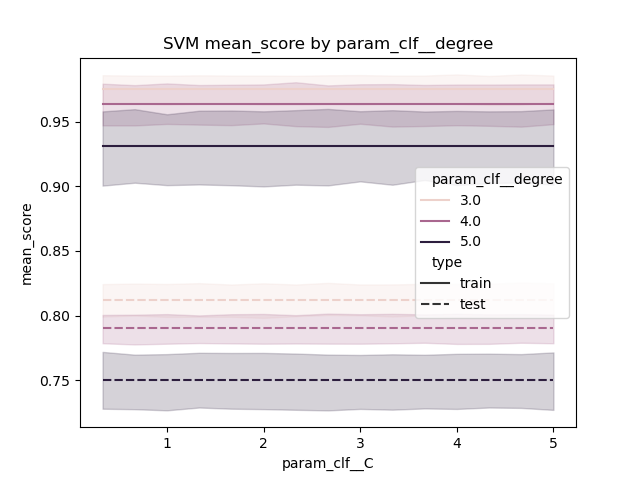
\includegraphics[width=.95\textwidth]{../results_second/svm/param_clf__degree_mean_score_param_clf__C.png}
      \caption{Polynomial SVM Degree Performance}
      \end{subfigure}%
    \begin{subfigure}{.5\textwidth}
      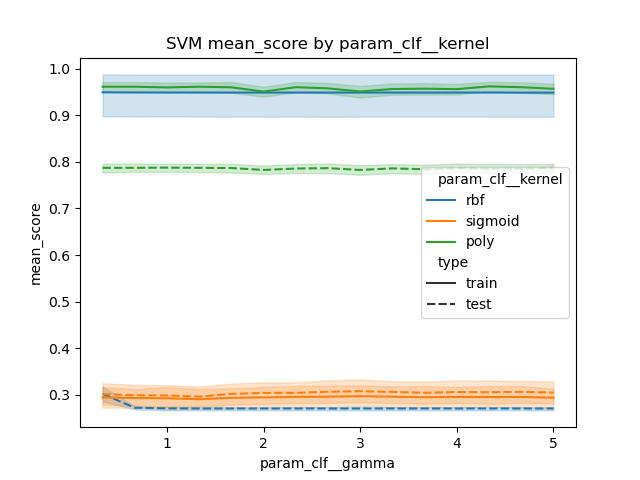
\includegraphics[width=.95\textwidth]{../results_second/svm/param_clf__kernel_mean_score_param_clf__gamma.png}
      \caption{Kernel Performance}
    \end{subfigure}
    \begin{subfigure}{.5\textwidth}
        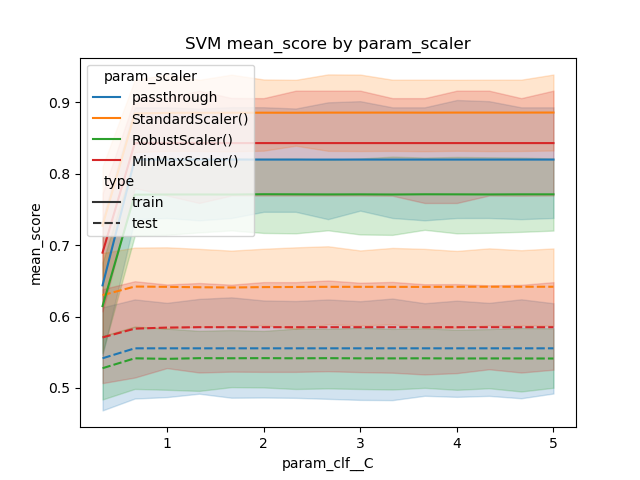
\includegraphics[width=.95\textwidth]{../results_second/svm/param_scaler_mean_score_param_clf__C.png}
        \caption{Preprocessing Performance for SVM} 
        \end{subfigure}%
      \begin{subfigure}{.5\textwidth}
        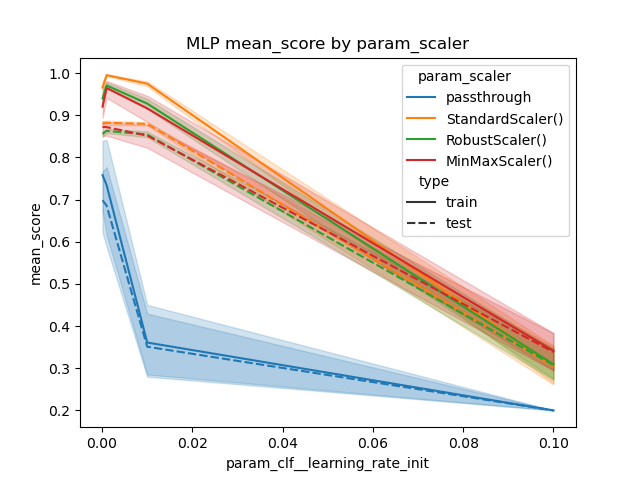
\includegraphics[width=.95\textwidth]{../results_second/mlp/param_scaler_mean_score_param_clf__learning_rate_init.png}
        \caption{Preprocessing Performance for MLPNet}
      \end{subfigure}
    \caption{Precursor Performance}
    \label{figure1}
\end{figure}

As we can see from these plots, the polynomial degree of 3 is best across the board (this was true at every step for every 
other parameter as well, the C parameter just looked the clearest). Likewise the standard scaler performed the best for SVM
and MLPNet (while also training faster!). Unfortunately I didn't feel like there was a clear cut best kernel because of 
the huge disparity in overfitting behavior between the different kernels. 

From all of this, I decided to do the following: I cut out all preprocessors other than the StandardScaler, all polynomial 
degrees other than degree of 3, and I restricted my search for gamma and C to be between .2 and 2 in steps of .2. Even with 
these simplifications, when I moved on to work with the full dataset it took over 8 hours. 

\section{Final Search}
I did my final search over the parameters explained above for the SVM, and I did 3 different MLPNet models with alpha from 
the list [0, .0001,.001,.01,.1] and a learning rate from the list [.0001, .001,.01,.1]. The 3 different MLPNet models are 
described by a list of their hidden layer sizes, and all used the same activation function. 

We can see the results of the gridsearch in Figure \ref{figure2}, and the best models in Table \ref{table1}. Since the 
parameters are cut off for size, I will provide the results here. Best SVM had a C of .2, gamma of 1.0, and the polynomial 
kernel. The best MLPNet model had an alpha of .0001, layout of [128,64,64,32], and a learning rate of .001.

\begin{figure}
    \begin{subfigure}{.5\textwidth}
      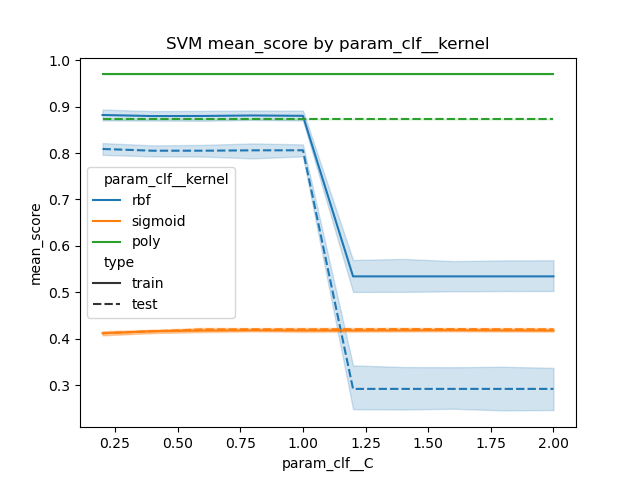
\includegraphics[width=.95\textwidth]{../results/svm/param_clf__kernel_mean_score_param_clf__C.png}
      \caption{SVM performance by C}
      \end{subfigure}%
    \begin{subfigure}{.5\textwidth}
      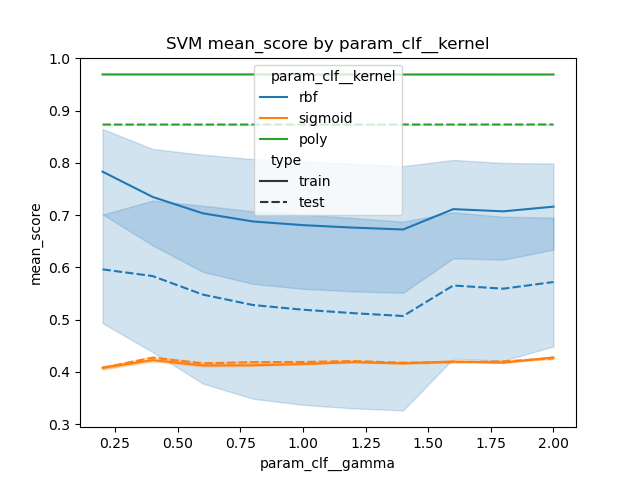
\includegraphics[width=.95\textwidth]{../results/svm/param_clf__kernel_mean_score_param_clf__gamma.png}
      \caption{SVM performance by gamma}
    \end{subfigure}
    \begin{subfigure}{.5\textwidth}
        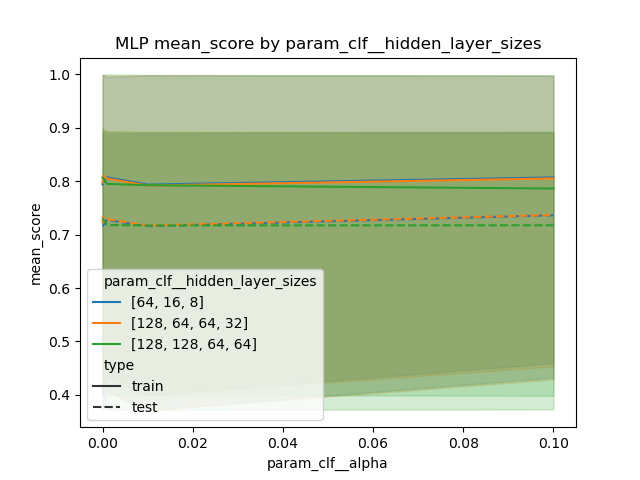
\includegraphics[width=.95\textwidth]{../results/mlp/param_clf__hidden_layer_sizes_mean_score_param_clf__alpha.png}
        \caption{MLP performance by alpha} 
        \end{subfigure}%
      \begin{subfigure}{.5\textwidth}
        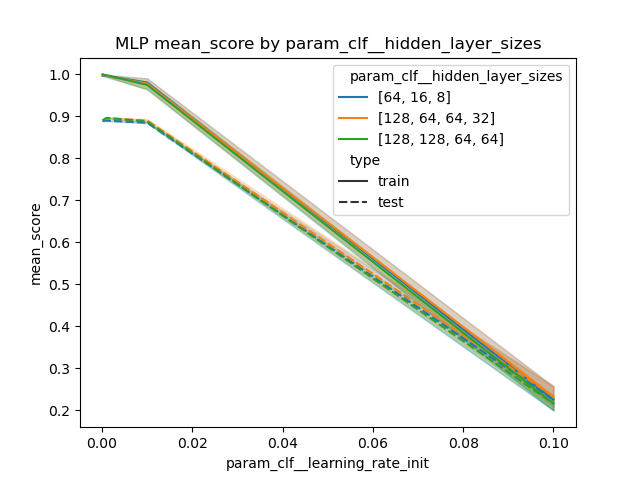
\includegraphics[width=.95\textwidth]{../results/mlp/param_clf__hidden_layer_sizes_mean_score_param_clf__learning_rate_init.png}
        \caption{MLP performance by learning rate}
      \end{subfigure}
    \caption{Full Data Search}
    \label{figure2}
\end{figure}

\begin{table}
    \resizebox*{.95\textwidth}{!}{\begin{tabular}{lllllll}
\toprule
{} &                   stack &                  NBbag &                 mlpbag &                  NBada &                treeada &                  SVMbag \\
\midrule
Index                       &                       2 &                    867 &                     14 &                     51 &                     47 &                      17 \\
mean\_fit\_time               &      1405.5506918430328 &     40.285290360450745 &      579.3783206343651 &     102.77094876766205 &      1229.745915234089 &      129.07705068588257 \\
std\_fit\_time                &       56.74206058134601 &     0.6317175670817758 &      7.455601391413241 &     0.8867015999451987 &     1.8724155730382983 &       9.796660667519168 \\
mean\_score\_time             &      11.178422927856445 &      51.00288212299347 &     0.5981229543685913 &     48.676812052726746 &      3.830958664417267 &      27.196506679058075 \\
std\_score\_time              &       1.405742496910865 &     1.8923625091969507 &    0.11387845129075089 &     1.8198226356237728 &    0.28462153313195493 &       4.294021210732005 \\
mean\_test\_accuracy          &                    0.79 &     0.5754999999999999 &                0.79525 &                  0.637 &                0.54825 &                 0.77575 \\
std\_test\_accuracy           &   0.0022360679774997916 &   0.019868316486305507 &   0.008525696452489974 &    0.01383835250309806 &     0.0067961386095341 &     0.00831790237980707 \\
rank\_test\_accuracy          &                       5 &                     44 &                      1 &                      1 &                      1 &                       2 \\
mean\_train\_accuracy         &      0.9977499999999999 &                0.62925 &     0.9940833333333333 &     0.8125833333333333 &                  0.764 &                 0.99425 \\
std\_train\_accuracy          &   0.0007592027982620297 &   0.004872684635347887 &  0.0009537935951883014 &    0.01061281981588514 &    0.01018713785995741 &   0.0008620067027324092 \\
mean\_test\_f1\_weighted       &      0.7912570496724283 &     0.5858494831502836 &     0.7949238630429338 &     0.6431246854754509 &     0.5576218846400178 &      0.7762111731817483 \\
std\_test\_f1\_weighted        &   0.0029872474406088608 &    0.01903181076309097 &   0.008385994462715676 &   0.012909250517893546 &   0.007753848653095678 &    0.009018811244895598 \\
rank\_test\_f1\_weighted       &                       3 &                     38 &                      1 &                      1 &                      1 &                       2 \\
mean\_train\_f1\_weighted      &      0.9977507823245164 &     0.6389193533117794 &     0.9940841593977978 &     0.8137017737836371 &     0.7653651061845691 &      0.9942576816522287 \\
std\_train\_f1\_weighted       &   0.0007583764213535456 &   0.005289021391854054 &  0.0009541156349656866 &   0.010307792046297188 &   0.010124753277141824 &   0.0008584699193975221 \\
mean\_test\_roc\_auc\_ovr       &      0.9730999015536933 &     0.9088672548387857 &     0.9749867328830162 &     0.9364586653065938 &     0.8743949551758458 &      0.9688421608215558 \\
std\_test\_roc\_auc\_ovr        &    0.000915550433627727 &   0.006604637647041263 &  0.0008938521311151068 &  0.0030788513632281837 &  0.0034540071161737835 &   0.0019750940256677376 \\
rank\_test\_roc\_auc\_ovr       &                       1 &                      1 &                      1 &                      1 &                      1 &                       1 \\
mean\_train\_roc\_auc\_ovr      &      0.9999612015765678 &     0.9389531956927522 &     0.9999600333256833 &     0.9844012423207428 &      0.949929571828595 &       0.999923288362849 \\
std\_train\_roc\_auc\_ovr       &  2.4671281578632394e-05 &  0.0030594180625836366 &  1.558742578374733e-05 &  0.0010215200718514444 &   0.002438923495362692 &  3.1182187144615235e-05 \\
best\_final\_test\_accuracy    &                    0.96 &                  0.602 &                  0.961 &                   0.75 &                  0.714 &                   0.791 \\
best\_final\_test\_roc\_ovr     &      0.9989464604987599 &      0.927274695189538 &      0.996860066599987 &     0.9706142287135784 &     0.9326248076880352 &      0.9701864899787338 \\
best\_final\_test\_f1\_weighted &      0.9600616632865854 &     0.6136405868499072 &     0.9609942113384318 &      0.752537870834654 &     0.7160316970317154 &      0.7909626666332018 \\
\bottomrule
\end{tabular}
}
    \caption{Best Results and MetaData}
    \label{table1}
\end{table}
  
\subsection{SVM Discussion}
I want to take a second and talk about how surprised I was that the polynomial model was the best, especially with 
the most simple degree. I was quite surprised to see that the legendary Radial Basis Function was so cleanly toppled, until 
I took a look at the compute times in \ref{figure3}. Looking back on the text output of the training cell, I can see that
a great many models timed out before they converged since I set the max iterations of the model to be 500. Moreover, we can 
see that the polynomial kernel was fit consistently the fastest. I think that this is evidence to support the idea that the 
polynomial kernel may not have necessarily been the best model for the job, just the model that converged the fastest to their
real optimal performance. 

\begin{figure}
    \begin{subfigure}{.5\textwidth}
      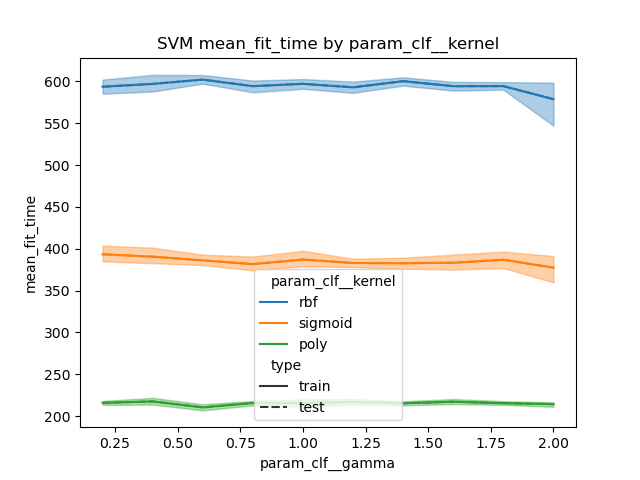
\includegraphics[width=.95\textwidth]{../results/svm/param_clf__kernel_mean_fit_time_param_clf__gamma.png}
      \caption{SVM Compute time by Gamma}
      \end{subfigure}%
    \begin{subfigure}{.5\textwidth}
      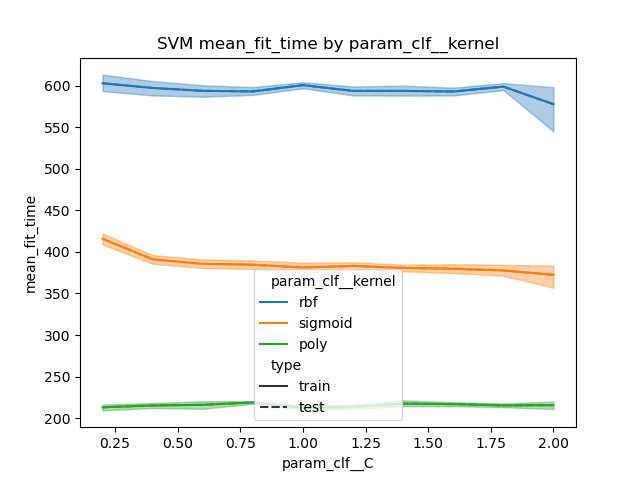
\includegraphics[width=.95\textwidth]{../results/svm/param_clf__kernel_mean_fit_time_param_clf__C.png}
      \caption{SVM compute time by C}
    \end{subfigure}
    \caption{Training time}
    \label{figure3}
\end{figure}

\section{Test Results}
The test results are also included in Table \ref{table1} in a manner that is consistent with all of my submissions this year,
since I am just using the same function. Interestingly, we can see that the MLPNet classifier outperformed the svm classifier
in every single metric I provided. I will take a moment to explicitly list all of the things that the MLPNet beat the SVM on:
Fit time, Score time, mean training score, training score consistency, mean validation score, validation score consistency,
final test score, and generalization. 

It is quite jarring just how solidly the MLPNet classifier out performed the SVM classifier, even with such a simple model. 
This model doesn't utilize any convolutional layers for feature extraction, and yet it is vastly superior to the svm model.
While I am not surprised that the MLPNet outperformed the SVM, I think that the degree with which it is outperforming is likely 
connected to the previously mentioned lack of covergence from the SVM classifier for the more classically promising parameters.

\subsection{Result examples}
To begin, I classified the samples into 4 groups: Both Difficult, Neither Difficult, MLP Difficult, and SVM Difficult. These 
describe samples which both models missclassified, neither models missclassified, only MLP missclassified, and only SVM missclassified.
We can see the requested scatter plot of the relative predicted probabilities of each class with the groups identified by color.

We can see from the scatter plots that the MLPNet classifier was much more likely to strongly assign a negative or positive 
probability for samples while the SVM was less confident. It seems like trousers are by far the easiest to identify, and that 
makes sense since they are the only item on this list which does not attempt to cover the torso. It also seems like pullover 
was the most difficult class, which is fair because even I wouldn't classify things as a pullover most of the time.

Jokes aside, it's pretty clear that the coat vs. pullover distinction is resting primarily on the activation of a center 
seam or zipper, which is a difficult one to catch on this scale.
\begin{figure}
    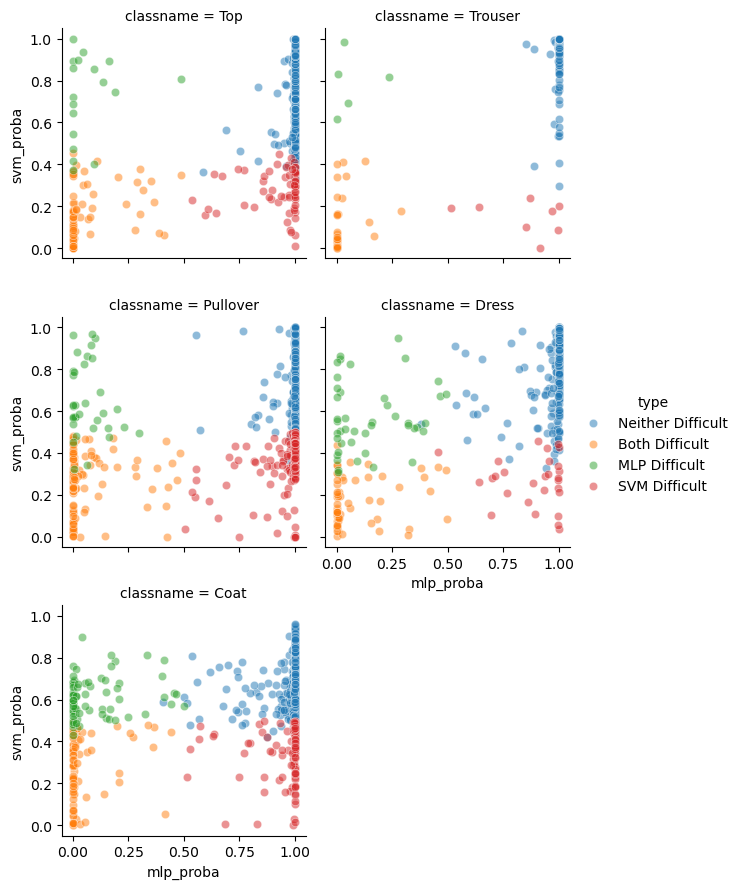
\includegraphics[width=.95\textwidth]{../results/difficulties.png}
    \caption{Probability Correlation}
    \label{figure4}
\end{figure}

\begin{figure}
    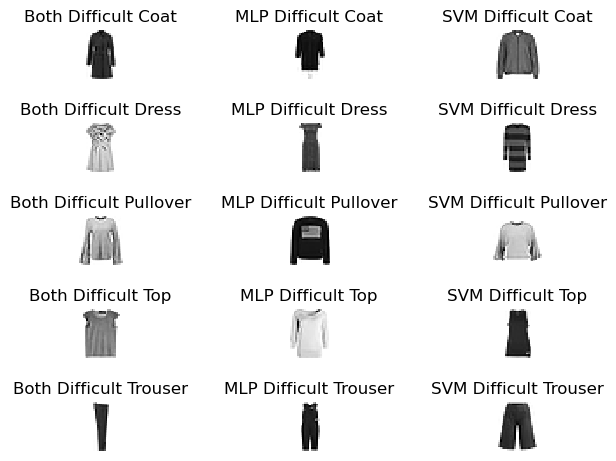
\includegraphics[width=.95\textwidth]{../results/Types_images.png}
    \caption{Example Misses}
    \label{figure5}
\end{figure}

\begin{table}
    \resizebox*{.95\textwidth}{!}{\begin{tabular}{llrrrrlrrlr}
\toprule
classname &           type &  index &  class &  svm\_proba &  svm\_call &  svm\_diff &  mlp\_proba &  mlp\_call &  mlp\_diff &  mean\_proba \\
\midrule
     Coat & Both Difficult &   4110 &      4 &   0.442786 &         3 &      True &   0.443113 &         3 &      True &    0.442950 \\
     Coat &  MLP Difficult &   4410 &      4 &   0.788874 &         4 &     False &   0.411459 &         2 &      True &    0.600166 \\
     Coat &  SVM Difficult &   4695 &      4 &   0.498579 &         2 &      True &   0.999999 &         4 &     False &    0.749289 \\
    Dress & Both Difficult &   3441 &      3 &   0.316876 &         0 &      True &   0.493340 &         0 &      True &    0.405108 \\
    Dress &  MLP Difficult &   3810 &      3 &   0.947275 &         3 &     False &   0.277057 &         1 &      True &    0.612166 \\
    Dress &  SVM Difficult &   3382 &      3 &   0.440828 &         4 &      True &   0.999520 &         3 &     False &    0.720174 \\
 Pullover & Both Difficult &   2801 &      2 &   0.399679 &         4 &      True &   0.485677 &         4 &      True &    0.442678 \\
 Pullover &  MLP Difficult &   2544 &      2 &   0.967783 &         2 &     False &   0.087898 &         4 &      True &    0.527840 \\
 Pullover &  SVM Difficult &   2877 &      2 &   0.498955 &         4 &      True &   0.999956 &         2 &     False &    0.749456 \\
      Top & Both Difficult &    436 &      0 &   0.347538 &         3 &      True &   0.487817 &         3 &      True &    0.417677 \\
      Top &  MLP Difficult &    921 &      0 &   0.807085 &         0 &     False &   0.488846 &         2 &      True &    0.647965 \\
      Top &  SVM Difficult &    137 &      0 &   0.429797 &         3 &      True &   0.983014 &         0 &     False &    0.706405 \\
  Trouser & Both Difficult &   1070 &      1 &   0.414774 &         3 &      True &   0.128738 &         3 &      True &    0.271756 \\
  Trouser &  MLP Difficult &   1914 &      1 &   0.815975 &         1 &     False &   0.236740 &         3 &      True &    0.526357 \\
  Trouser &  SVM Difficult &   1974 &      1 &   0.202755 &         4 &      True &   1.000000 &         1 &     False &    0.601378 \\
\bottomrule
\end{tabular}
}
    \caption{Difficult Items MetaData and Correct Call Probability}
    \label{table2}
\end{table}

\begin{table}
  \resizebox*{.95\textwidth}{!}{\begin{tabular}{llrrrrrrrrrrr}
\toprule
classname &           type &  index &  svm\_Top &  svm\_Trouser &  svm\_Pullover &    svm\_Dress &  svm\_Coat &      mlp\_Top &  mlp\_Trouser &  mlp\_Pullover &    mlp\_Dress &     mlp\_Coat \\
\midrule
     Coat & Both Difficult &   4110 & 0.005298 & 3.400359e-03 &      0.042683 & 5.058327e-01 &  0.442786 & 2.365100e-08 & 2.130062e-08 &  1.573007e-08 & 5.568867e-01 & 4.431132e-01 \\
     Coat &  MLP Difficult &   4410 & 0.030210 & 1.239151e-02 &      0.121701 & 4.682354e-02 &  0.788874 & 4.298497e-03 & 6.602311e-05 &  5.829506e-01 & 1.226316e-03 & 4.114585e-01 \\
     Coat &  SVM Difficult &   4695 & 0.000140 & 1.433529e-05 &      0.501266 & 6.572349e-07 &  0.498579 & 3.423842e-10 & 1.651771e-09 &  7.073309e-07 & 4.242566e-09 & 9.999993e-01 \\
    Dress & Both Difficult &   3441 & 0.634818 & 8.693196e-03 &      0.032233 & 3.168760e-01 &  0.007380 & 5.066321e-01 & 1.002960e-05 &  1.814361e-05 & 4.933395e-01 & 2.181102e-07 \\
    Dress &  MLP Difficult &   3810 & 0.005804 & 3.739344e-02 &      0.003378 & 9.472747e-01 &  0.006150 & 5.968212e-08 & 7.229427e-01 &  9.305746e-14 & 2.770572e-01 & 1.495911e-15 \\
    Dress &  SVM Difficult &   3382 & 0.016419 & 5.340160e-03 &      0.068409 & 4.408281e-01 &  0.469004 & 6.118283e-10 & 9.267762e-10 &  5.577999e-09 & 9.995196e-01 & 4.804015e-04 \\
 Pullover & Both Difficult &   2801 & 0.010303 & 6.220486e-03 &      0.399679 & 9.726465e-02 &  0.486532 & 1.175790e-06 & 3.336376e-06 &  4.856768e-01 & 1.669695e-05 & 5.143020e-01 \\
 Pullover &  MLP Difficult &   2544 & 0.000001 & 4.374569e-07 &      0.967783 & 1.306642e-07 &  0.032215 & 5.591335e-08 & 2.054001e-09 &  8.789789e-02 & 2.023371e-08 & 9.121020e-01 \\
 Pullover &  SVM Difficult &   2877 & 0.000220 & 1.417864e-04 &      0.498955 & 1.571403e-04 &  0.500526 & 6.485726e-10 & 2.794313e-08 &  9.999561e-01 & 4.390890e-05 & 1.202809e-09 \\
      Top & Both Difficult &    436 & 0.347538 & 1.203015e-02 &      0.117837 & 4.216860e-01 &  0.100909 & 4.878167e-01 & 3.265101e-10 &  3.229960e-03 & 5.089526e-01 & 7.274153e-07 \\
      Top &  MLP Difficult &    921 & 0.807085 & 2.450316e-02 &      0.096842 & 6.291166e-02 &  0.008659 & 4.888463e-01 & 5.221946e-06 &  5.098310e-01 & 1.317414e-03 & 4.320292e-10 \\
      Top &  SVM Difficult &    137 & 0.429797 & 6.534917e-03 &      0.007387 & 5.379585e-01 &  0.018323 & 9.830143e-01 & 1.932584e-04 &  9.893235e-07 & 1.679147e-02 & 2.352449e-08 \\
  Trouser & Both Difficult &   1070 & 0.003292 & 4.147736e-01 &      0.008784 & 5.595047e-01 &  0.013646 & 7.145541e-06 & 1.287379e-01 &  1.998690e-05 & 8.712345e-01 & 4.990616e-07 \\
  Trouser &  MLP Difficult &   1914 & 0.005595 & 8.159752e-01 &      0.002692 & 1.665820e-01 &  0.009156 & 1.048266e-11 & 2.367398e-01 &  1.773124e-09 & 7.632602e-01 & 4.216483e-11 \\
  Trouser &  SVM Difficult &   1974 & 0.022238 & 2.027554e-01 &      0.305108 & 6.706847e-02 &  0.402830 & 3.543663e-12 & 1.000000e+00 &  4.664057e-12 & 3.572991e-08 & 8.299836e-12 \\
\bottomrule
\end{tabular}
}
  \caption{Difficult Items Full Calls}
  \label{table3}
\end{table}
As for visualizing some samples of each group, I decided to picture the image for each combination of class and difficulty
type which had the highest average confidence. I decided that it would likely be more interesting to look at the images which
evoked some genuine misunderstanding from our models, rather than randomly selected images.

My discussion of these items will (mostly) go in order of the table, which correlates to the reading order of the grid of images.
I will not cover every single image, since that will result in far more verbosity than I want to write and you want to read.

Starting off with the first image of Both Difficult Coat, neither of our models were very confident. They both called this one a dress, which I'd
say is a valid interpretation. I don't think I would've noticed this image is a coat if I'm honest. However, when I consulted 
my wife she immediately identified it as a coat without even being prompted on what classes we can choose from, so possibly 
my personal fashion ability needs more training data.

Moving on to MLP Difficult Coat, this is likely due to the behavior I discussed earlier about how coats will look like pullovers
with a seam in the middle. This item's seam is very small and poorly rendered, and the image shows some strange noise at the bottom.
As such, MLPNet called this a pullover likely due to it's sensitivity, where these small errors weren't enough to throw off the 
less sensitive SVM.

Skipping to Both Difficult Dress, I highly suspect the design of the dress around the chest which has been absolutely murdered
by compression threw off both of them. Very few details can be made out at all from this image which out models likely relied on.

Skipping to SVM Difficult Dress, I believe the horizontal line pattern caused the SVM to say that this is a coat. This actually 
makes a lot of sense to me because I see way more coats with this kind of pattern than I do dresses. MLPNet is sensitive enough 
to draw a conclusion from the shape of the item, while the SVM likely was thrown off by the lines.

Skipping down to MLP Difficult Pullover, I think it's obviously the american flag that's being difficult here. The MLP classifier 
had no idea how to handle this, and somehow that ended up with it being a coat. I wonder if this sample set is biased towards having 
more coats with designs than pullovers. This error would require more in-depth research to debug. Possibly it's more common 
to put a flag on a coat than a pullover.

Skipping down to Both Difficult Top, I think that the wavy folds and lack of sleaves of the top made this too similar to a dress, 
which both of out models called. Admittedly, they both gave the Top a pretty high confidence for a missed call, with MLP 
being almost 50/50 between dress and top.

Skipping to SVM Difficult Trouser, this was classified as a coat by the SVM. My theory as to why is because it expands down from 
the top, which if we look at SVM Difficult Pullover seems to be a feature that the SVM associated more strongly with coats. I find 
it more interesting that MLP gave a perfect 100\% probability that this image is trousers, which is rare to see.



Finally, for Both Difficult Trouser... I have to agree with the models on this one. These are not pants, this is a pant, singular.
This does show evidence that a common feature the SVM and the MLPNet identified is that pants should have 2 legs. I'm quite 
interested, however, in how confident the SVM was in calling the incorrect item, since the incorrect item overcame a confidence
of .41. Looking back at the full probabilities for each item included in Table \ref{table3}, we can see that this sample had 
called Dress at .559. 

\end{document}